The first construction in the proof of Theorem \ref{thm:3stein4} is a 3--handlebody regular neighbourhood of the 1--skeleton of our Stein complex $S$.
Put $G$ to be the 1--skeleton of $S$ and $A\subset G$ a maximal spanning tree.
We know that $G$ is a graph where, for any vertex $v$ of $G$, $\deg_G v$ is 3 if $v$ is boundary and 4 if it is interior.

We first triangulate the building blocks of Figure \ref{fig:3thickeningblocks} and display them in Figure \ref{fig:3thicktri}.
Each block in Figure \ref{fig:3thicktri} depicts one view of a triangulated 2--sphere.
The blocks have symmetry that should be clear, and the full triangulated block is found by taking the cone on the triangulated 2--sphere depicted.
Note that each edge block is actually a triangulated prism, and the only difference between the blocks is the set of marked boundary curves.
The proof of Theorem \ref{thm:3stein4} is procedural in its creation of handlebodies, and the details for the triangulated case are contained in Algorithm \ref{alg:4handlebody}.
In this section we use the notation laid out in the proof of Theorem \ref{thm:3stein4}, and we take $A\subset G$ to be fixed throughout.

The result of Algorithm \ref{alg:4handlebody} includes strips inside of solid tori $V$ used to compute 0--framing curves.
When the strip is an annulus, the curve is found as one of the boundary components of the annulus.
When it is a M\"obius strip, there is one boundary component $2\lambda$.
We take $2\Lambda$ halfway around its length to one full longitude of $V$, and perform one last positive half twist in order to get an actual 0--framing curve $\lambda$.
To be precise, the half twist is a curve $\gamma$ in the meridian direction of the boundary of $V$ connecting the endpoints of $\frac{1}{2}(2\lambda)$, and the positive direction is the anticlockwise direction determined by the $\II^2$ fibers over the boundary component of $U_S(G)$.

\begin{algorithm}
	\caption{Building the 4--handlebody of the 1--skeleton of the Stein complex}
	\label{alg:4handlebody}
	\KwData{a Stein complex $S$}
	\KwResult{a triangulated 4--manifold $A_4$ that is the 4--thickening of $U_S(G)$, a set of trianglated solid tori $\mathcal{V}$ in the boundary over which we will attach 2--handles, and a set of strips $\mathcal{C}$ in the boundary tori of $\mathcal{V}$ used to determine 0--framings as in the proof of Theorem \ref{thm:3stein4}}
	\Begin{
		$A_3,C\longleftarrow\emptyset$\;
		\ForEach{vertex $v$ of $A$}{
			add the triangulated vertex block $v_B$ associated to the type of vertex $v$ is in $S$ to $A$\;
			add the triangulated red curve in the boundary of $v_B$ depicted in Figure \ref{fig:3thicktri} to $C_A$\;
		}
		\ForEach{edge $e=(u,v)$ of $A$}{
			attach the triangulated edge block $e_B$ associated to the type of edge $e$ is in $S$ over the blocks $u_B$ and $v_B$\;
			add the triangulated red curve in the boundary of $e_B$ depicted in Figure \ref{fig:3thicktri} to $C_A$\;
			combine the curves in $C_A$ over identical boundaries\;
		}
		$A_4\longleftarrow$ result of Algorithm \ref{alg:nthickening} with input $A_3$\;
		$C_A\longleftarrow$ the inclusions of $C_A$ into the copies of $A_3$ at $A_3\times\{\pm1\}$ in $A_4$\;
		\ForEach{edge $e=(u,v)$ of $e(G)\setminus e(A)$}{
			$e_B\longleftarrow$ the triangulated edge block associated to the type of edge $e$ is in $S$\;
			$E_B\longleftarrow$ the result of Algorithm \ref{alg:nthickening} on $e_B$\;
			attach $E_B$ over the thickenings $U_B$ and $V_B$ of $u_B$ and $v_B$ in $A_4$ in the unique orientation preserving way\;
			add the pair of triangulated red curves from Figure \ref{fig:3thicktri} included into the copies of $e_B$ at $e_B\times\{\pm 1\}$ in $E_B$ to $C_A$\;
			combine the curves in $C_A$ over identical boundaries\;
		}
		$\mathcal{V},\mathcal{C}\longleftarrow\emptyset$\;
		\ForEach{curve $c$ of $C_A$}{
			$V\longleftarrow\emptyset$, to be the solid torus associated with $c$\;
			$C\longleftarrow\emptyset$, to be the strip in $V$ that determines 0--framing\;
			\ForEach{thickened 4--prism $P_i^4$ intersecting $c$ nontrivially}{
				$P_0^3,P_1^3\longleftarrow$ the identical walls of $P_i^4$, themselves 3--prisms, intersecting $c$ in an edge\;
				$P^2\longleftarrow$ the identical wall shared by $P_0^3,P_1^3$, itself a 2--prism\;
				add $P_0^3,P_1^3$ to $V$\;
				add $P^2$ to $C$\;				
			}
			combine the elements of $V$ over identical boundaries\;
			add $V$ to $\mathcal{V}$\;
			combine the elements of $C$ over identical boundaries\;
			add $C$ to $\mathcal{C}$\;
		}
	}	
\end{algorithm}

\begin{figure}
	\centering
	\captionsetup{justification=centering}
	\caption{The triangulated blocks used in the 3--thickening of the 1--skeleton of the Stein complex}
	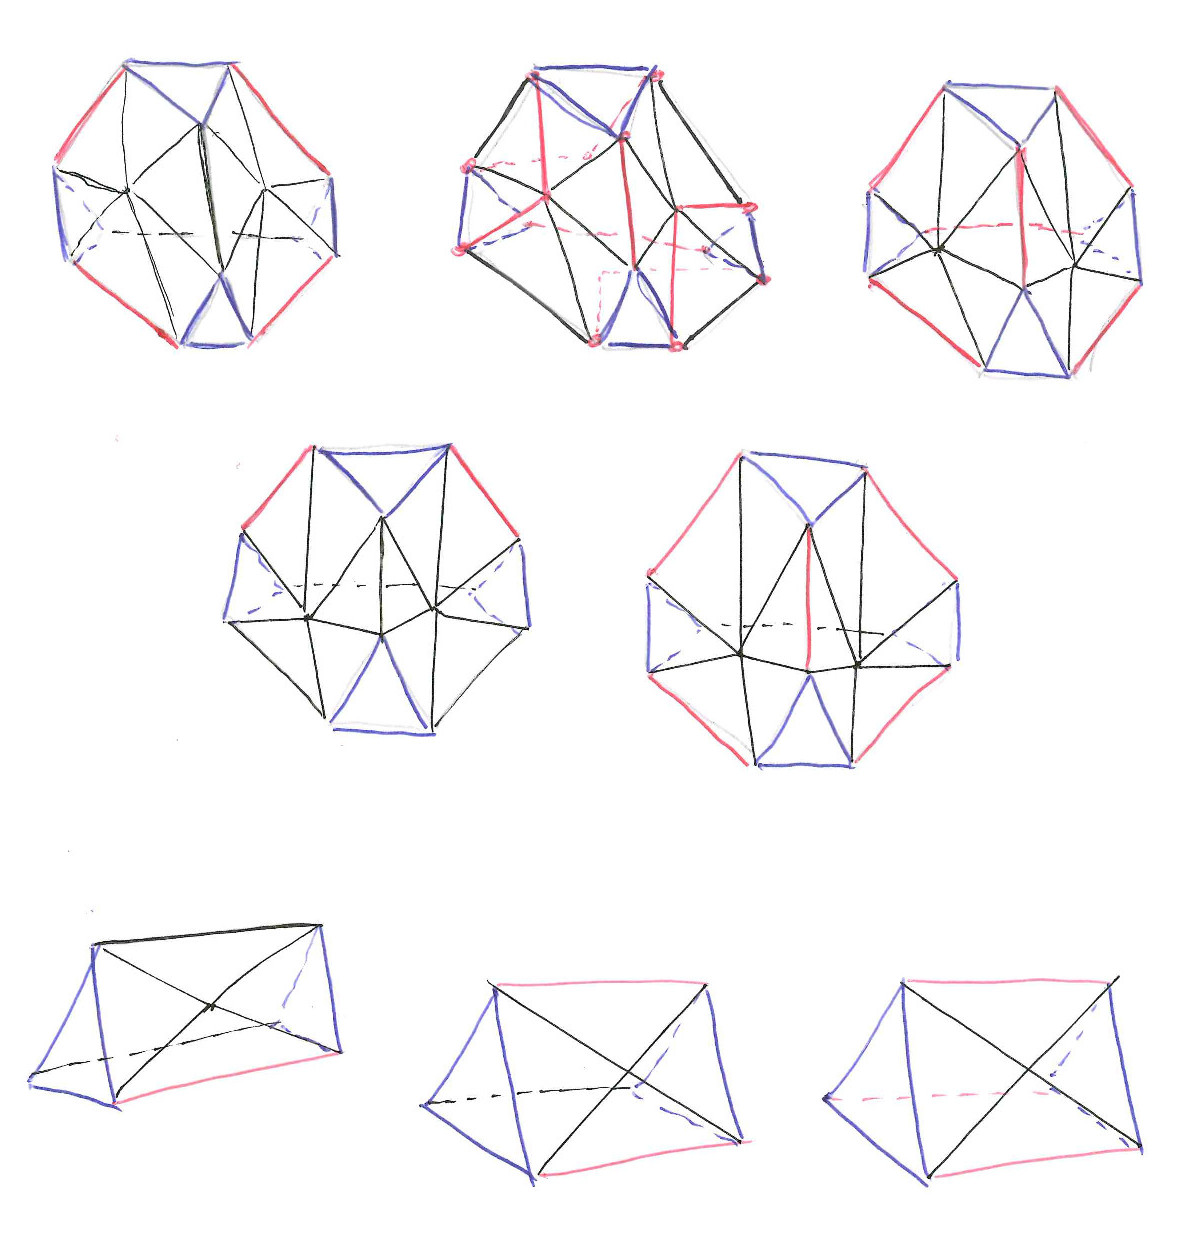
\includegraphics[width=6in]{figures/3thicktri.jpg}
	\label{fig:3thicktri}
\end{figure}